\documentclass{article}
\usepackage[utf8]{inputenc}
\usepackage[english]{babel}

\DeclareUnicodeCharacter{2212}{-}

\usepackage{amsfonts}
\usepackage{amsthm}
\usepackage{amssymb}
\usepackage{amsmath}
\usepackage{tikz}
\usetikzlibrary{shapes.arrows,chains,trees}

\theoremstyle{definition}
\newtheorem{definition}{Definition}[section]
\newtheorem{theorem}{Theorem}[section]
\newtheorem{hypothesis}{Hypothesis}[section]
\newtheorem{example}{Example}[section]

\newcommand{\G}{\mathcal{G}}

\setlength{\parindent}{0pt}

\begin{document}

\tableofcontents
\pagebreak

\section{Problems}
Firstly we shall look at two problems which belong to the complexity class NP.

\textbf{Traveling Sales Person}\\
Consider a finite set $N$ of cities; $\{1, 2 \dots n\}$. The distance, or cost,
of traveling between cities $i$ and $j$ is given by $D(i,j)$ where $D$
is a symmetric matrix.

$$\forall\ i, j\quad D(i,J) \in \mathbb{N}\quad D(i,j) = D(j,i)$$

The problem is to find a path, or permutation, of
cities where each city appears exactly once in the path and the total
cost is minimised.

The brute force solution is to consider all paths, doing this would require
considering $!n$ paths.

\textbf{Boolean Formula Satisfiability}\\
A boolean formula consists of the logical binary operators $(\land, \lor, \neg)$
and a finite set of variables $X$ where each variable can be either true or false.
The problem consists of deciding if there exists a set of values for the variables $X$
which results in the boolean formula being true.

$$(x_1 \land x_2) \land \neg x_3$$

$$(x_1 \land x_2) \land \neg x_1$$

A brute force solution would be to consider all $2^{|X|}$ possible assignments.

The link between these two problems is the na\"ive brute force solution is not
tractable for large values of $n$.

\begin{itemize}
    \item \textbf{Input}: Real numbers $x_1,\dots x_n$
    \item \textbf{Output}: Yes iff there exists a subset of $x_i$ which sum to 1.
\end{itemize}

\textit{Traveling Sales Person}\\
\begin{itemize}
    \item \textbf{Inputs}:
    \item \textbf{Output}:
\end{itemize}
Consider a finite set $N$ of cities; $\{1, 2 \dots n\}$. The distance, or cost,
of traveling between cities $i$ and $j$ is given by $D(i,j)$ where $D$
is a symmetric matrix.

$$\forall\ i, j\quad D(i,J) \in \mathbb{N}\quad D(i,j) = D(j,i)$$

The problem is to find a path, or permutation, of
cities where each city appears exactly once in the path and the total
cost is minimised.

The brute force solution is to consider all paths, doing this would require
considering $!n$ paths.

\textit{Traveling Sales Person (Yes-No Version)}\\
\begin{itemize}
    \item \textbf{Inputs}:
    \item \textbf{Output}:
\end{itemize}
Consider a finite set $N$ of cities; $\{1, 2 \dots n\}$. The distance, or cost,
of traveling between cities $i$ and $j$ is given by $D(i,j)$ where $D$
is a symmetric matrix.

$$\forall\ i, j\quad D(i,J) \in \mathbb{N}\quad D(i,j) = D(j,i)$$

The problem is to find a path, or permutation, of
cities where each city appears exactly once in the path and the total
cost is minimised.

\textit{Boolean Formula Satisfiability}\\
\begin{itemize}
    \item \textbf{Inputs}:
    \item \textbf{Output}:
\end{itemize}
A boolean formula consists of the logical binary operators $(\land, \lor, \neg)$
and a finite set of variables $X$ where each variable can be either true or false.
The problem consists of deciding if there exists a set of values for the variables $X$
which results in the boolean formula being true.

$$(x_1 \land x_2) \land \neg x_3$$

$$(x_1 \land x_2) \land \neg x_1$$

A brute force solution would be to consider all $2^{|X|}$ possible assignments.

The link between these two problems is the na\"ive brute force solution is not
tractable for large values of $n$.

\textit{Knapsack Problem}\\
\begin{itemize}
    \item \textbf{Input}: Real numbers $x_1,\dots x_n$
    \item \textbf{Output}: Yes iff there exists a subset of $x_i$ which sum to 1.
\end{itemize}

The following is in conjunctive normal form:
$$(x_1 \lor x_2) \land \neg x_3$$
The following is not in conjunctive normal form;
however it is in \textit{disjunctive normal form}
$$(x_1 \lor x_2) \lor \neg x_3$$
This is because there is the negation on the left hand side of the logical or.

\begin{definition}
    Given an undirected graph $\mathcal{G}$ which is a pair of vertices and edges $(V,E)$,
    a subset of vertices $S \subset V$ is a \textit{clique} iff
    $$\forall\ x, y \in S\ \exists\ \textrm{an edge}\ (x,y) \in E$$
\end{definition}

\begin{definition}
    If $S$ is a clique in $\mathcal{G}$ and $|S| = q$ then $S$ is called a \textit{$q$-clique}.
\end{definition}

An obvious consequence of this definition is that for any edge $(x,y)$ there is a 2-clique.

\begin{definition}
    The \textit{$q$-clique problem} is finding if there exists a $q$-clique in a given graph
    $\mathcal{G}$ where $q \in \mathbb{N}$.
\end{definition}

\textbf{Distinctness problem: upper bound}\\
\begin{itemize}
    \item \textbf{Input}: $(x_0, x_1,\dots x_n) \in \mathbb{R}^n$
    \item \textbf{Output}: Yes iff $\forall\ i,j$ where $0 \leq i,j \leq n, i \neq j$ we have $x_i \neq x_j$
\end{itemize}


\pagebreak
\section{Turing Machines}
\subsection{Deterministic Turing Machines}
%TODO
What do Turing machines do? Why are we looking at them?
Conceptually a turing machine is a \textit{tape} which is infinite in both directions,
the input is writen on this tape with the rest of the tape being blank. We have a head
which can read and write to the tape. The machine moves across the tape acording to
a transition function until it reaches a terminal state which produces a yes or no result.

\begin{center}
    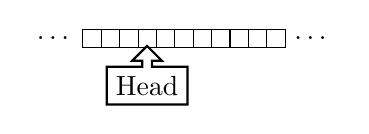
\begin{tikzpicture}[
            start chain=1 going right,start chain=2 going below,node distance=-0.15mm
        ]
        \node [on chain=1] at (-1.5,-.4) {\ldots};
        \foreach \x in {1,2,...,11} {\x, \node [draw,on chain=1] {}; }
        \node [
            name=k,
            arrow box,
            on chain=2,
            arrow box arrows={north:.25cm},
            draw=black,thick
            ] at (-0.335,-1) {Head};
        \node [name=r,on chain=1] {\ldots};
    \end{tikzpicture}
\end{center}

\begin{definition}
    Formally a Turing machine consists of
    \begin{itemize}
        \item A \textit{tape alphabet} $\Gamma$ $\{a_1, a_2 \dots a_n, \beta\}$,
            where $a_i$ is a symbol, and $\beta$ is the blank or empty symbol.
        \item An \textit{input alphabet} $\Sigma$
            where $\Sigma \subset \Gamma \setminus \{\beta\}$.
        \item A set of states $Q$ $\{q_0, q_1 \dots q_m, q_y, q_n\}$ where $q_0$ is the
            initial state, $q_y$ is the terminal yes state, and $q_n$ is the terminal no state.
            $Q\prime = Q \setminus \{q_y,q_n\}$, i.e. the non-terminal states.
        \item A transition function $\delta$,
            where $\delta\ :\ (Q\prime \times \Gamma) \rightarrow
            (Q \times \Sigma \times \{L,S,R\})$.
            What this means is we look at a pair of a non-terminal state
            and a symbol from the alphabet;
            given this we enter a new state $q \in Q$,
            we write to the tape a symbol $a \in \Gamma$,
            and we stay or move the head left or right $(\{L,S,R\})$.
    \end{itemize}
\end{definition}

\begin{definition}
    Given an input $n$ and a Turing machine,
    $T(n)$ is the amount of times the transition function 
    $\delta$ must be applied to reach a terminal state.
\end{definition}

\textbf{Even or odd}
\begin{example}
    In this example we will present a turing machine to decide if a number is even.
    \begin{itemize}
        \item Input: a number $x \in \mathbb{Z}$ in unary form; i.e. $\{1 = X, 2 = XX\dots\}$,
            thus $\Sigma = \{X\}$.
        \item Output: yes iff $x$ is even, otherwise no. I.e. the turing machine will finish
            in state $q_y$ iff $x$ is even.
        \item Transition function $\delta$ is described as a matrix below with the states
            $Q\prime = \{q_0,q_1\}$ and $\Sigma = \{X,\beta\}$,
            output is $(Q \times \Sigma \times \{L,S,R\})$.
            \begin{center}
                \begin{tabular}{ c c c }
                    & $q_0$           & $q_1$           \\
                    X    & ($q_1,\beta,R$) & ($q_0,\beta,R$) \\
                    $\beta$ & ($q_y,\beta,S$) & ($q_n,\beta,S$) \\
                \end{tabular}
            \end{center}
    \end{itemize}
    For this Turing machine $T(n) = n + 1$.
\end{example}

\textbf{Recognising Palindromes}\\
A palindrome is any word such that the reversed word is equal to the word itself,
consider the alphabet $\Gamma = \{a,b\}$, examples of palindromes would be $a, aa, aba$ etc.
Can we construct a Turing machine which recognises palindromes for the alphabet $\Gamma$?

We can, we simply move forward and backward checking each letter at opposite ends is the same,
until the entire word has been checked.
This means for palindromes $T(n)$ is equal to $n + (n - 1) \dots + 1$. Thus
$$T(n) = \frac{n^2 + n}{2}$$

However in non palindrome cases, say $aaa \dots ab$, then $T(n)$ is very small.

\subsection{Non-Deterministic Turing Machines}
\begin{definition}
    \textit{Nondeterministic Turing Machine (NTM)} has
    the same constituent elements as a deterministic Turing Machine,
    the difference between TM and NTM is in the way they work.
    NTM has a “guessing module” with write-only head attached to it.
    Before NTM starts working, an input word is written on a tape;
    the working head observes cell 1; guessing head observes cell −1.
    NTM works in two stages:
    \begin{enumerate}
        \item \textbf{Guessing stage}
            Guessing head moves along the tape from right to left
            shifting to the next cell on each step.
            On each step guessing head writes a letter from $\Gamma$ on the tape.
            The process may or may not terminate.
            During this stage the control module of NTM and its working head remain passive;
            NTM is not in any “state”. When (if ever) the guessing state terminates, NTM moves to the second stage.
        \item \textbf{Verifying stage}
            NTM adopts the initial state $q_0$ and works as ordinary TM
            with the combination of the “guessed word” and the original input word, as its input.
            During this second stage the guessing module and its guessing head are passive.
    \end{enumerate}
    \textbf{Observe}
    \begin{itemize}
        \item For a fixed input word $x$, the sequence of steps from stages (1) and (2) is called computation for $x$.
        \item NTM accepts an input $x$ if there exists a computation (for $x$) ending with the state $q_Y$.
        \item If NTM accepts $x$ there might also be computations (for $x$) ending with $q_N$.
        \item There might be many computations (for $x$) leading to $q_Y$.
    \end{itemize}
\end{definition}
\begin{definition}
    Let NTM accept $x$.
    Complexity of accepting $x$ is the number of steps in the shortest accepting computation for x.
\end{definition}
\begin{definition}
    Complexity of NTM is the function
    \begin{equation}
        T(n) = max\ \left\{
            \begin{array}{@{}ll@{}}
                m \textrm{ such that there exists }x\textrm{ where} |x| = n\\
                \textrm{ such that the complexity of accepting }x\textrm{ is }m
            \end{array}\right\}.
    \end{equation}
    If such $x$ does not exist let $T(n) = 1$.
\end{definition}

\subsection{$O, \Omega, \Theta$ Notation}
\begin{definition}
    Given a computation $T(x)$ where $|x| = n$,
    constants $c > 0$ and $n_0 > 0$,
    and functions $f_1, f_2, f_3$ defined on $n$,
    we have
    \begin{itemize}
        \item $O(f_1(n))$ where $\forall\ |x| \geq n_0$ we have $f_1(n) \leq c\,T(x)$
        \item $O(f_1(n))$ describes the upper bound for $T(x)$.
        \item $\Omega(f_2(n))$ where $\forall\ |x| \geq n_0$ we have $f_2(n) \geq c\,T(x)$
        \item $\Omega(f_2(n))$ describes the lower bound for $T(x)$.
        \item $\Theta(f_3(n))$ where we have both $O(f_3(n))$ and $\Omega(f_3(n))$,
            or relying on the fact that $O(g(n))$ and $\Omega(g(n))$ are sets of functions, we can define
            $$\Theta(g(n)) \equiv O(g(n)) \cap \Omega(g(n))$$
        \item $\Theta(f_3(n))$ describes the exact bound of for $T(x)$.

    \end{itemize}
\end{definition}


\section{$O, \Omega, \Theta$ Notation}

\begin{definition}
	$O(n)$
\end{definition}

\begin{definition}
	$\Omega(n)$
\end{definition}

\begin{definition}
	$\Theta(n)$
\end{definition}
Bit on worst case vs average vs best case

Note that for some $n$ $T(n)$ will be very small and for others it will be much larger,
usually this leads us to consider the complexity of the Turing machine to be 


\pagebreak
\section{Polynomial Transformations and Equivalence}
\textbf{Polynomial Transformations}
\begin{definition}
    Consider two languages $\mathcal{L_1} \subset A_1$ and $\mathcal{L_2} \subset A_2$,
    $\mathcal{L_1}$ is said to be \textit{polynomially transformable} to $\mathcal{L_2}$ if
    $$\exists\ f : A_1 \rightarrow A_2$$
    such that $f$ can be computed with polynomially complexity and $f$ preserves the language. I.e.
    $$\forall\ x \in A_1\ x \in \mathcal{L_1}\ \mathrm{iff}\ f(x)\in \mathcal{L_2}$$
\end{definition}

Practically $\mathcal{L_1} \propto \mathcal{L_2}$ means that
$\mathcal{L_2}$ is not harder than $\mathcal{L_1}$;
i.e. if $\mathcal{L_2} \in P$ then $\mathcal{L_1} \in P$.
Furthermore this relation is transitive.
$$
  \mathcal{L_1} \propto \mathcal{L_2},\ 
  \mathcal{L_2} \propto \mathcal{L_3},\Rightarrow
  \mathcal{L_1} \propto \mathcal{L_3}
$$

\textbf{Polynomial Equivalence}
\begin{definition}
    If we have two languages such $\mathcal{L_1} \propto \mathcal{L_2}$ and
    $\mathcal{L_2} \propto \mathcal{L_1}$, then they are said to be \textit{polynomially equivalent}.
    Thus we have $\mathcal{L_1} \approx \mathcal{L_2}$.
\end{definition}
This is an equivalence as such it is reflexive, symmetric, and transitive;
as such $\forall\ R,\ S,\ T$:
\begin{itemize}
    \item $R \approx R$
    \item if $R \approx S$ then $S \approx R$.
    \item $
        R \approx S,\ 
        S \approx T \Rightarrow
        R \approx T
        $
\end{itemize}

%%TODO
In practise what this means is that we can see what problem a class is in if we can
polynomially translate it to another problem in a known class; for example:
$$
  \forall\ \mathcal{L_1} \in P\ 
  \forall\ \mathcal{L_2} \in P\ 
  \mathcal{L_1} \approx \mathcal{L_2}
$$


\pagebreak
\section{Complexity Class P and NP}
\subsection{Class P}
\begin{definition}
    \textit{Class P} is the class of all Yes - No computational problems
    (languages) $L$ such that there exists $TM$ and a polynomial $p(n)$ such that
    $TM$ solves $L$ with complexity $T(n) \leq p(n)$ for all $n \geq 1$.
\end{definition}
\textbf{Examples}
\begin{itemize}
    \item “Even unary non-negative numbers” is in P , take $n + 1$ as polynomial $p(n)$ from the definition
    \item “Palindromes” is in P, $p(n) = cn^2$ for a large enough positive constant $c$
    \item “Primality” is in P . This is a problem of deciding for a given integer number $n > 0$,
        represented in decimal (or binary) form, whether $n$ is prime
    \item “Traveling Salesman” and “Satisfiability” are \textit{probably} not in P, but no proofs for any of them are known
\end{itemize}

\subsection{Class NP}
We say that NTM solves the Yes - No problem $L$ if it accepts exactly all Yes inputs in $L$.
\begin{definition}
    \textit{Class NP} consists of Yes - No problems (languages) $L$ such that
    there exist polynomial $p(n)$ and NTM for solving $L$ with complexity $T(n) \leq p(n)$ for any $n \geq 1$.
    \textbf{Examples}
    \begin{itemize}
        \item Travelling Salesman $\in$ NP.
            To show this, we need to construct a NTM for solving this problem with polynomial complexity.
            On the guessing stage the NTM produces an arbitrary permutation of cities,
            and on the verifying stage, working like an “ordinary” TM,
            checks whether the length of the guessed tour does no exceed the boundary $B$.
            An accepting computation for an input $x$ exists if and only if there is a short tour.
            This computation consists in writing out a guess and finding the corresponding sum of all distances.
            Clearly the complexity of this computation is polynomial.
            According to the definition, a non-accepting computation does not contibute to the complexity.
        \item Boolean satisfiability $\in$ NP.
            NTM first guesses a satisfying assignment of truth values to variables,
            and then verifies the guess in polynomial time.
    \end{itemize}
\end{definition}

\begin{theorem}
    $P \subset NP$
\end{theorem}
\begin{proof}
    Let $L$ be a Yes-No problem from P,
    and M be a (deterministic) TM for solving L in polynomial time.
    We get a NTM for solving $L$ in polynomial time by imitating $M$ on the verification stage
    and ignoring the guessing stage.
    The question whether P = NP, is a famous open problem.
\end{proof}

\begin{theorem}
    Let $L \in NP$,
    then there exist a polynomial $p(n)$ and TM for solving $L$ with complexity $O(2^{p(n)})$.
\end{theorem}
\begin{proof}
    Let $N$ be an NTM for solving $L$ with complexity $TN (n) \leq r(n)$
    where $r(n)$ is a polynomial.
    By the definition of NTM, for every accepted input $x$ with $|x| = n$
    there is a guess word in the tape alphabet $\Gamma$ of the length not greater than $r(n)$
    such that $N$ adopts the state $q_Y$ in no more than $r(n)$ steps.
    The total number of possible guesses is less than $|\Gamma|r(n)+1$
    Now we construct a (deterministic) TM $M$ as follows.
    $M$ examines every possible guess in turn,
    and for each of them runs the verification stage of $N$ up to $r(n)$ steps.
    That will take $$O(r(n)|\Gamma|r(n))$$ steps.
    By the definition of O-symbol, that’s the same as $O(2p(n))$ for a certain polynomial $p(n)$.
\end{proof}

\section{Structure of the Class NP}
Recall that it is not known whether or not P = NP, the widely accepted hypothesis being that this equality is wrong.
Let NPC ⊂ NP denote the class of all NP-complete problems,
and denote NPI := NP \ (NPC ∪ P).
Theorem. If P \neq NP, then:
\begin{itemize}
    \item NPI \neq \varnothing;
    \item there exist the problems A,B \in NPI such that neither A \propto B, nor B \propto A.
        Proof is nontrivial.
        The item (2) of the Theorem states that under the hypothesis P \neq NP the set NPI is divided into more that one equivalence classes with respect to polynomial transformation.
\end{itemize}

2. Complements to languages
Definition. Let L ⊂ Σ∗ be a language over an alphabet Σ. The set of words L = Σ∗ \ L
is called the complement to L.
Observe that L is not necessarily a language, i.e. a set of words generated by a grammar (or accepted by a TM). For all problems from NP the complement is indeed a language, however it is not at all obvious that if L ∈ NP, then L ∈ NP. That is because the definition of NTM (unlike the definition of Yes - No TM) is non-symmetrical with respect to Yes - No output.
Example. For the problem CNF SAT, the complement is the following Yes - No prob- lem.
Input: Boolean formula F in conjunctive normal form.
Output: Yes if F is not satisfiable (i.e., identically false), else No.
There is no apparent way of taking advantage of the non-determinism (i.e., guessing module) for solving this problem. It seems to be nothing essentially better than just examining one by one every true/false assignment to all variables and checking whether it gives the value false to F .

\subsection{Class co-NP}
Definition
 (1) co−NP ={L: L∈NP}; (2) co−P={L: L∈P};
 Hypothesis. NP ̸= co−NP.
This hypothesis is “stronger” than P ̸= NP since obviously P = co−P, thus if
P = NP, then NP = co−NP.
Theorem. Let L be an NP-complete problem such that L ∈ NP. Then NP = co−NP.
Proof is relatively straightforward. We don’t consider it in this course.
4. Some famous candidates for problems in NPI
(1) Graph Isomorphism
Input: Two graphs G = (V, E) and G′ = (V ′, E′).
Output: Yes if there is a bijective (one-to-one) map (function), called isomorphism, f: V −→V′ suchthat(v,w)∈Eisequivalentto(f(v),f(w))∈E′;elseNo.
The status of Graph Isomorphism is unknown. Despite many efforts no polynomial time algorithm was found. On the other hand, the problem seems to be too “rigid” to be NP-complete. Compare it with the following NP-complete problem Isomorphism to Subgraph.
Input: Two graphs G = (V, E) and G′ = (V ′, E′).
Output: Yes if there is a subgraph in G which is isomorphic to G′; else No.
Isomorphism to Subgraph is NP-complete problem which is proved by polynomially transforming to it the k-clique problem (take as G′ the complete graph with k vertices).
(2) Linear Programming
Input : System of linear inequalities in several variables with integer coefficients. Output : Yes if the system is consistent (i.e., has a solution) in real numbers, else No.
The status of Linear Programming was open for a long time until in late seventies a polynomial-time algorithm was discovered. Even before that it seemed quite unlikely for the problem to be NP-complete since the complement to Linear Programming is in NP (follows from so-called Duality Theorem in linear programming). If Linear Programming was NP-complete, then, by Theorem from previous section, NP = co−NP, which is probably wrong.

\subsection{NP-hard problems}
Definition. A search problem L is NP-hard if for any language L′ ∈ NP the following holds:
L′ ∝T L. (∗∗) Theorem. A search problem L is NP-hard if and only if for at least one (thus, for any)
NP-complete language L′ relation (∗∗) is true.
Proof. If L is NP-hard, then for any language from NP, in particular, for any NP- complete language L′ the relation (∗∗) is true.
Conversely, if there exists an NP-complete language L′ such that (∗∗) is true, then for any language L′′ ∈ NP we have
L′′ ∝ L′ ∝T L,
which, by Theorems 1 and 2 of Section 8, implies that L′′ ∝T L, thus L is NP-hard by
the definition.
Example. Consider a modification of Travelling Salesman problem as a search problem in which the output is the tour of the smallest length. Call this modification Optimal Travelling Salesman (OptTS), as opposed to Yes - No modification (TS) which involves a threshold.oTheorem. TS ∝T OptTS, therefore OptTS is N P -hard.
Proof. The OTM for TS with threshold B first uses the oracle to solve the OptTS with the same set of cities and distances as the input of TS (one step of computation), then in polynomial time finds the length l of the produced optimal tour and checks whether B ≥ l. If the latter inequality is true, then the answer is Yes, else – No.
Observe that this example does not use the relation ∝T in full force, addressing the oracle only once.

\subsection{NP-Complete Problems}
\begin{definition}
	$\mathcal{L}$ is \textit{NP-Complete} if
	\begin{itemize}
		\item $\mathcal{L} \in NP$
		\item $\forall\ \mathcal{L\prime} \in NP\ \mathcal{L\prime} \propto \mathcal{L}$
	\end{itemize}
\end{definition}

What does this definition mean?
Any two NP-complete languages are polynomially equivalent.
Any NP-Complete problem is at least as hard as any other problem in NP.

\begin{theorem}
	Given two languages $\mathcal{S}, \mathcal{T} \in NP$,
	if $\mathcal{S} \in NPC$ and $\mathcal{S} \propto \mathcal{T}$ then
	$\mathcal{T} \in NPC$.
\end{theorem}

This theorem is rather useful for proving that a language is NP-Complete,
however it leaves us with the issue of proving a first language is NP-Complete.

\begin{definition}
	A boolean formula $F$ is in \textit{conjunctive normal form} if it is in the form
	\begin{equation}
	\begin{split}
		F &= f_1 \land f_2 \dots \land f_n \\
		f_i &= y_1 \lor y_2 \dots \lor y_m \\
		y_j &= x\ |\ \neg x
	\end{split}
	\end{equation}
\end{definition}

The following is in conjunctive normal form:
$$(x_1 \lor x_2) \land \neg x_3$$
The following is not in conjunctive normal form;
however it is in \textit{disjunctive normal form}
$$(x_1 \lor x_2) \lor \neg x_3$$
This is because there is the negation on the left hand side of the logical or.

\begin{definition}
	Given an undirected graph $\mathcal{G}$ which is a pair of vertices and edges $(V,E)$,
	a subset of vertices $S \subset V$ is a \textit{clique} iff
	$$\forall\ x, y \in S\ \exists\ \textrm{an edge}\ (x,y) \in E$$
\end{definition}

\begin{definition}
	If $S$ is a clique in $\mathcal{G}$ and $|S| = q$ then $S$ is called a \textit{$q$-clique}.
\end{definition}

An obvious consequence of this definition is that for any edge $(x,y)$ there is a 2-clique.

\begin{definition}
	The \textit{$q$-clique problem} is finding if there exists a $q$-clique in a given graph
	$\mathcal{G}$ where $q \in \mathbb{N}$.
\end{definition}



\pagebreak
\section{Cook’s Theorem}

\subsection{Formulation}
\begin{theorem}
    Boolean Satisfiability problem is NP-complete.
\end{theorem}
Actually we will prove that CNF-satisfiability problem is NP-complete.

\subsection{Proof}
\subsection{Formulation}

The following is in conjunctive normal form:
$$(x_1 \lor x_2) \land \neg x_3$$
The following is not in conjunctive normal form;
however it is in \textit{disjunctive normal form}
$$(x_1 \lor x_2) \lor \neg x_3$$
This is because there is the negation on the left hand side of the logical or.

\begin{definition}
    Given an undirected graph $\mathcal{G}$ which is a pair of vertices and edges $(V,E)$,
    a subset of vertices $S \subset V$ is a \textit{clique} iff
    $$\forall\ x, y \in S\ \exists\ \textrm{an edge}\ (x,y) \in E$$
\end{definition}

\begin{definition}
    If $S$ is a clique in $\mathcal{G}$ and $|S| = q$ then $S$ is called a \textit{$q$-clique}.
\end{definition}

An obvious consequence of this definition is that for any edge $(x,y)$ there is a 2-clique.

\begin{definition}
    The \textit{$q$-clique problem} is finding if there exists a $q$-clique in a given graph
    $\mathcal{G}$ where $q \in \mathbb{N}$.
\end{definition}


%\pagebreak
%\section{Knapsack Problem}
\begin{definition}
    \begin{itemize}
        \item \textbf{Input}: Real numbers $x_1,\dots x_n$
        \item \textbf{Output}: Yes iff there exists a subset of $x_i$ which sum to 1.
    \end{itemize}
\end{definition}


\pagebreak
\section{Approximate Algorithms}
Many important practical problems are in NP-hard,
we need a tractable solution for them.
It may be the case that we can find an algorithm for our relevant cases.
Alternatively we may need to solve the problem for the input
data of a relatively small size, so that even an exponential-time algorithm is acceptable.
Finally, we can try to solve the problem approximately;
i.e. solve the problem as close to optimally as possible but accept some degree of error
or incorrectness.
This last approach is suitable for optimization search problems.\\

\textbf{Examples of optimization search problems}
\begin{itemize}
    \item Travelling Salesperson (find the smallest tour)
    \item Find the largest clique in a graph
    \item Vertex Covering (find the smallest covering)
\end{itemize}

\subsection{Ratio bound and relative error}
For approximation algorithms we need an \textit{objective function}
which will allow us to measure the difference of the approximate and optimal algorithms.\\

For example in the traveling sales person problem,
the objective function is the length of the tour produced by the algorithm.
We want to determine how "close" our approximate algorithm is to the optimal one.
We will assume that the objective function is always positive.

\begin{definition}
    Let $C$ denote the value of the objective function at our approximate solution,
    and $C\prime$ at an optimal solution.
\end{definition}

\textbf{Ratio Bound}
\begin{definition}
    An approximation algorithm has \textit{ratio bound} $\rho(n)$
    if for any input of the size $n$ the value $C$ of the objective function
    at the approximate solution satisfies the inequality
    $$max(C/C\prime, C\prime/C) \leq \rho(n)$$
\end{definition}

Observe that
$$ 0 < C \leq C\prime $$
thus for maximization problems
$$ max(C/C\prime, C\prime/C) = C\prime/C $$
and for minimization problems
$$ max(C/C\prime, C\prime/C) = C/C\prime $$

Observe that $\rho(n) \geq 1$,
and secondly that when $\rho(n) = 1$ we have an optimal solution.
By definition a large  ratio bound (might) means that the approximate
solution is much worse than an optimal one.
Usually $\rho(n)$ is a constant,
i.e. the ratio bound does not grow with the size of the input.\\

\textbf{Relative Error Bound}
\begin{definition}
    For $C, C\prime$ and $n$  the \textit{relative error bound $\epsilon(n)$} is defined as
    $$\frac{abs(C - C\prime)}{C\prime} \leq \epsilon(n)$$
\end{definition}

\textbf{Approximation algorithm for Vertex Covering}\\
Recall that the vertex covering problem is defined as such
\begin{itemize}
    \item \textbf{Input}:
        a graph $\G,\ (V,E)$
    \item \textbf{Output}:
        a set $S \subset V$ such that $\forall\ (v,w) \in E$
        either $v$ or $w$ are in $S$.
        I.e. every vertex is reachable,
        and the fewest possible vertices are in $S$.
\end{itemize}

\textbf{Algorithm}
\begin{enumerate}
    \item Let $S$ be $\varnothing$
    \item Let $E\prime$ be the set of edges $E$
    \item While $E\prime$ is non-empty
        \begin{enumerate}
            \item
                Let $(v,w)$ be an arbitrary edge of $E\prime$
            \item
                Let $S$ be $S \cup \{v,w\}$
            \item
                Remove from $E\prime$ every edge having either $v$ or $w$ as a vertex
        \end{enumerate}
    \item Return the set $S$ as the vertex covering

\end{enumerate}

\textbf{Properties of the Algorithm}
\begin{enumerate}
    \item The algorithm is correct
    \item The algorithm has polynomial complexity
    \item The algorithm $\rho(n) = 2$
\end{enumerate}
\textbf{Proof}
\begin{proof}
    Let $A$ denote the set of all edges that are chosen by the algorithm.
    No two edges of $A$ have a common vertex,
    since once the edge $(v, w)$ is chosen,
    all edges having either $v$ or $w$ as vertices are deleted.
    Thus, each new execution adds exactly two new vertices to $S$, thus $|S| = 2|A|$.
    The optimal covering $S\prime$, by definition, must cover every edge in $A$.
    Hence
    \begin{align*}
           S\prime &\supset A \\
         |S\prime| &\geq |A|\\
         |S\prime| &\geq |S|/2\\
        2|S\prime| &\geq |S|\\
                 2 &\leq |S|/|S\prime|\\
                   &\leq C/C\prime \\
           \rho(n) &= 2
    \end{align*}
\end{proof}

\textbf{Approximation algorithm for Travelling Salesperson with triangle inequality}\\
\begin{itemize}
    \item \textbf{Input}:
        A matrix $d_{ij}$ such that $\forall\ i,j\, d(i,j) > 0$ and $\forall\ i,j,k$
        $$d(i,j) \leq d(i,k) + d(k,j)$$
    \item \textbf{Output}:
        A permutation $i_1, i_2,\dots i_m$ (called “tour”) of such that the following sum is minimised.
        $$\sum_{1\leq x < m} d(x,x+1)$$
\end{itemize}
Travelling Salesman with triangle inequality is NP-hard.\\

\textbf{Algorithm for $\Delta$Traveling Salesperson}\\
Given a connected graph $\mathcal{G}\ (V,E)$,
\begin{enumerate}
    \item
        Choose a vertex $v \in V$, to serve as the root of a tree.
        Build a spanning tree $T$ beginning at $v$;
        note that this can be done in polynomial time using Prim's or Kruskal's algorithm.
    \item
        Perform a pre-order walk on the tree $T$ returning the list of nodes as a tour.
\end{enumerate}

We can now propose three properties of this algorithm:
\begin{enumerate}
    \item It is correct
    \item It has polynomial complexity
    \item It has a ratio bound $\rho(n) = 2$
\end{enumerate}

\begin{proof}
    Let $L*$ denote an optimal tour,
    $d(L)$ be the length of $L$,
    $d(L*)$ be the length of $L*$.
    Observe that a spanning tree for $\G$ can be obtained by deleting any edge from any tour.
    Thus, for a minimal spanning tree $T$,
    with sum of weights on all edges $d(T)$,
    the following inequality holds
    $$d(T) \leq d(L*)$$
    Let W be a Full Walk of $T$,
    and $d(W)$ be its length.
    Since $W$ visits every edge of $T$ exactly twice,
    $$d(W ) = 2d(T )$$
    It follows that
    $$d(W) \leq 2d(L*)$$
    By the triangle inequality,
    Preorder Walk L is not longer than $W$:
    $$d(L) \leq d(W)$$
    As a result, we have:
    \begin{align*}
        d(L) &\leq 2d(L*)\\
        d(L) &\leq 2d(L*), d(L)/d(L*) wu 2 \\
        \rho(n) &= 2
    \end{align*}
\end{proof}

\textbf{No Ratio Bound for Traveling Salesperson}\\
\begin{theorem}
    If P $\neq$ NP then there is no
    approximation algorithm for general Travelling Salesman with polynomial complexity
    and constant ratio bound.
\end{theorem}

\begin{proof}
%We show how to solve Hamiltonian Cycle (HC) problem in polynomial time using a hypothetical approximation algorithm, with polynomial complexity and constant ratio bound ρ, for general Travelling Salesman (TS), as a subroutine.
%Let G = (V, E) be an input of HC. Construct an input of TS with the set of cities V and the distance function:
%d(u, v) = 1 if (u, v) ∈ E
%d(u, v) = ρ|V | + 1 if (u, v) ∈/ E.
%Clearly, this input of TS can be constructed from G in polynomial time.
%If G contains a hamiltonian cycle, then its length will be |V |. If G does not contain a hamiltonian cycle, then there is a pair (u,v) of subsequent cities in any tour such that (u, v) ∈/ E, thus the size of any tour will be at least
%(ρ|V | + 1) + (|V | − 1) = (ρ + 1)|V | > ρ|V |.
%Thus, we can decide whether G contains a hamiltonian cycle by approximately solving the instance of TS. If the size of the solution tour is ≤ ρ|V |, then G contains a hamiltonian cycle, else G has no hamiltonian cycles.
\end{proof}



\pagebreak
\section{Complexity Lower Bounds}
\begin{definition}
    A function $L(n)$ is called a \textit{complexity lower bound}
    for a computational problem $L$
    in a given class $M$ of models of computation
    if for any algorithm from $M$ which solves $L$ with complexity $T(n)$ the following relation holds:
    $$T(n) = \Omega(L(n))$$
\end{definition}

Finding non-trivial lower bounds is an important part of a comprehensive analysis of an algorithm,
which might save time spent on trying to construct a better algorithm.
Very few natural problems have proven lower bounds in the class of all Turing machines because these models are powerful.
An example of the quadratic lower bound for the problem of recognizing palindromes in the class of one-tape,
one-head Turing machines was mentioned earlier in this unit.
If we assume $P \neq NP$ hypothesis, then any polynomial serves as a lower bound for any NP-complete problem in the class of all Turing machines.
Clearly it should be easier to prove lower bounds for narrower classes $M$ of algorithms.
On the other hand such a class should be “natural enough” for the lower bound to be of some practical use.
This part of Lecture Notes describes a general method for proving complexity lower bounds for algebraic computation trees.

\subsection{A Lower Bound for Comparison Sorting}
We can arrive at a lower bound for comparison based for sorting using decision trees.

As input we have a finite set of items to sort
and a binary relation $\leq$ where we have $\forall\ a,b,c:$
\begin{itemize}
    \item Reflexivity: $a \leq a$
    \item Anti-Symmetry: if $a \leq b$ and $b \leq a$ then $a = b$
    \item Transitivity: if $a \leq b$ and $b \leq c$ then $a \leq c$
\end{itemize}

\begin{example}
The most obvious example is less than equal on the integers
$$1 \leq 1 \leq 2 \leq 74782$$
$$1 \leq 74782$$
\end{example}

We will use any given binary relation as the basis of our decision tree,
at each node of the tree we compute one binary relation
the left child will represent the result of the computation being true
conversely the right child will mean the computation result was false.
$$$$
Consider sorting three items $(a,b,c)$ we can derive a decision tree showing that
there exists a lower bound complexity for comparison sorting.

\begin{center}
    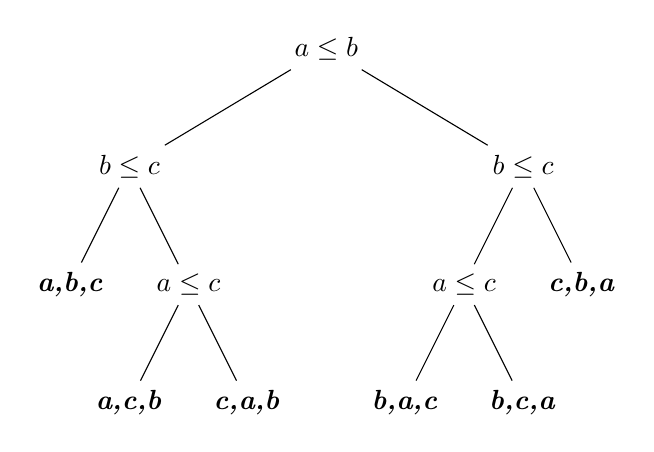
\begin{tikzpicture}[level distance=1.5cm,
  level 1/.style={sibling distance=5cm},
  level 2/.style={sibling distance=1.5cm},
  level 3/.style={sibling distance=1.5cm}]
  \node {$a \leq b$}
    child {node {$b \leq c$}
        child {node {\textbf{\textit{a,b,c}}}}
        child {node {$a \leq c$} {
          child {node {\textbf{\textit{a,c,b}}}}
          child {node {\textbf{\textit{c,a,b}}}}
      }}
    }
    child {node {$b \leq c$}
        child {node {$a \leq c$} {
          child {node {\textbf{\textit{b,a,c}}}}
          child {node {\textbf{\textit{b,c,a}}}}
      }}
          child {node {\textbf{\textit{c,b,a}}}}
    };
\end{tikzpicture}
\end{center}

Observe that the height or depth of the tree represents the amount of computations which must be performed.
Furthermore observe that the height of the tree is not the same for every root,
for the ordering \textbf{\textit{b,a,c}} we have height three
and for \textbf{\textit{a,b,c}} we have height two.
This is because we can prune some branches due to the transitive property of $\leq$,
given $a \leq b$ and $b \leq c$ we also know that $a \leq c$ is true.
Thus we do not need to compute $a \leq c$.
Conversely given $a \leq b$ and $c \leq b$ we \textbf{do not know} that $a \leq c$ is true.
This is another computation we need to perform to have a correct ordering.
Obviously this tree is correct for $n = 3$, so we can say
the complexity lower bound for $n = 3$ is 3 computational steps.
This is because equipped with only comparison we can only go in one
of two directions after each computation (true or false),
and we must be able to produce all six possible orderings.

How do
How many branches can we prune?

Well for a three item set $(a,b,c)$ there exists precisely $!3 = 6$ orderings;
thus our decision tree 
or more generally there exists for an $n$ item set $!n$ orderings.
Because
$$\Omega(n log n)$$


\subsection{Algebraic computation trees: examples}
We can expand the decision tree model to something more powerful

Consider the problem of finding if a point is inside the unit circle
\begin{itemize}
    \item Input: a point $(x,y) \in \mathbb{R}^2$
    \item Output: yes iff $x^2 + y^2 \leq 1$
\end{itemize}
The complexity of this algorithm (the height of the tree) is 4, i.e., a constant.
This is quite natural since we assume that the size of the input is a constant.
\begin{center}
    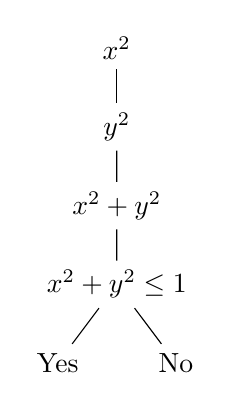
\begin{tikzpicture}[level distance=1cm,
  level 1/.style={sibling distance=2cm},
  level 2/.style={sibling distance=1.5cm},
  level 3/.style={sibling distance=1.5cm},
  level 4/.style={sibling distance=1.5cm},
  level 5/.style={sibling distance=1.5cm}]
  \node {$x^2$}
        child {node {$y^2$}
        child {node {$x^2 + y^2$}
        child {node {$x^2 + y^2 \leq 1$}
            child {node {Yes}}
            child {node {No}}
            }}
        };
\end{tikzpicture}
\end{center}

To further generalise our algebraic computation trees,
we will say that every node, except leaves, have three children.
The children correspond to the computation being
\begin{enumerate}
    \item $(= 0)$
    \item $(< 0)$
    \item $(> 0)$
\end{enumerate}
In the example below for the sake of space and brevity we don't show all the different branches,
simply because we never make any changes to our computation dependent on the result;
that is until the very end where we use it for our yes or no result.
This tree, were it completed, would have $3^4 = 81$ nodes,
much more than our previous tree.
However observe that the height remains unchanged at four,
thus the complexity is the same.

\begin{center}
    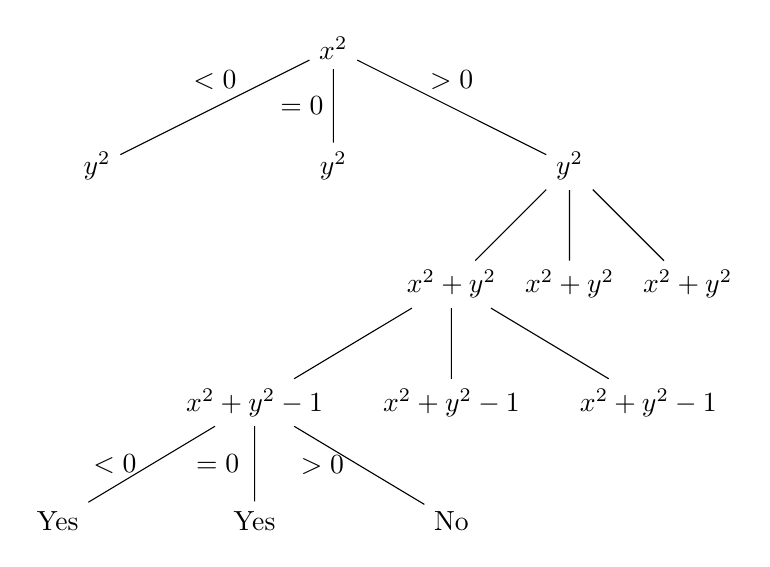
\begin{tikzpicture}[level distance=1.5cm,
  level 1/.style={sibling distance=3cm},
  level 2/.style={sibling distance=1.5cm},
  level 3/.style={sibling distance=2.5cm},
  level 4/.style={sibling distance=2.5cm}]
    \node {$x^2$}
            child {node {$y^2$} edge from parent node[left,above=3pt] {$< 0$}
            }
            child {node {$y^2$} edge from parent node[left] {$= 0$}
            }
            child {node {$y^2$}
                child { node {$x^2 + y^2$} 
                    child { node {$x^2 + y^2 - 1$} 
                        child { node {Yes} edge from parent node[left=2pt] {$< 0$}}
                        child { node {Yes} edge from parent node[left=2pt] {$= 0$}}
                        child { node {No}  edge from parent node[left=2pt] {$> 0$}}
                    }
                    child { node {$x^2 + y^2 - 1$} }
                    child { node {$x^2 + y^2 - 1$} }
                }
                child { node {$x^2 + y^2$} }
                child { node {$x^2 + y^2$} }
            edge from parent node[left,above=3pt] {$> 0$} }
       ;
\end{tikzpicture}
\end{center}

\begin{example}
    One can generalise this example from membership of the unit circle to membership
    of the $n$ dimensional unit ball.
    Simply calculate
    $$1 \leq \sum_{i=1}^{n} x_i^2$$
    You calculate $x_i^2$ for the $i$-th dimension and add it to the running total;
    this takes $2n$ steps.
    In case $n = 2$ we get complexity four as our computation tree showed.
\end{example}

\subsection{Algebraic computation trees: definition}
\begin{definition}
    A subset $S \subset R^n$ is called \textit{(basic) semi-algebraic} if it is defined by
    $$\{P_1(x_1,\dots x_n) = 0,\dots P_n\}
    \cup
    \{Q_1(x_1,\dots x_n) > 0,\dots Q_m\}$$
    where $P_i$ and $Q_j$ are polynomials in $n$ variables
    i.e., S is a set of all solutions of a system of equations and strict inequalities.
\end{definition}

Algebraic computation tree $T$ in variables $x_1,\dots x_n$
is a tree with the root $v_0$ such that to every vertex $v$ (except leaves)
is an arithmetic operation (addition, subtraction or multiplication) 
and a polynomial $f_v$ is attached.

For example $f_3 = f_1 + f_2$ where $f_3$ is the new polynomial;
more precisely in our previous example membership of the unit circle
we have
$$f_1 = x^2 \quad f_2 = y^2 \quad f_3 = x^2 + y^2$$
$$f_4 = f_3 - 1 = x^2 + y^2 - 1$$

Let $v_0, v_1,\dots, v_\omega$ be the sequence of vertices
along the (unique) branch leading from the root $v_0$ to $v_\omega$.
An arithmetic operation at $v_i$ is performed on a pair from
$$\{x_1,\dots x_n\} \cup \{f_0\dots f_{i - 1}\}$$
and the result is at $f_i$.
Note that every $v$ has exactly three children
$$(> 0, = 0, < 0)$$

Let $*_i \in \{>0,=0,<0\}$ for $0 \leq i < \omega$ be the sign of $f_{v_i}$,
One can assign the semi-algebraic set $U_\omega$ to $v_\omega$
$$U_\omega = \{f_0*_00,f_1*_10\dots f_{\omega - 1} *_{\omega - 1}0\}$$

To each leaf $\omega$ of $T$ an output Yes or No is assigned.
We call $U_\omega$ an accepting set if the leaf $\omega$ has the output Yes assigned.
We say that T tests the membership to the union of all accepting sets.

The computation process works as follows.
A specific point $x \in \mathbb{R}^n$ is taken as an input.
Then the value $f_{v_0}(x)$ is computed and the sign of this value is determined.
According to the sign, the algorithm goes to the corresponding child $v_1$ of $v_0$.
If the process eventually arrives to a Yes-vertex, then $x$ belongs to an accepting set,
and, therefore, to the union of all accepting sets.

\subsection{Distinctness problem: upper bound}
\begin{itemize}
    \item \textbf{Input:} $(x_0, x_1,\dots x_n) \in \mathbb{R}^n$
    \item \textbf{Output:} Yes iff $\forall\ i,j$ where $0 \leq i,j \leq n, i \neq j$ we have $x_i \neq x_j$
\end{itemize}
An immediate solution for this problem is to sort the numbers $(x_0, x_1,\dots x_n)$
then compare pairwise neighbours for equivalence; this has complexity $O(nlogn)$.
It is clear that this algorithm can be represented in a form of algebraic computation tree
of the height $O(nlogn)$ (compare with sorting).
We are going to develop a general method for proving lower complexity bounds for algebraic computation trees,
and will apply this method to prove the $\Omega(nlogn)$ lower bound for Distinctness.
Unlike the very elementary proof of $\Omega(nlogn)$ for sorting,
for Distinctness no elementary proof is known.

\subsection{Connected components of semialgebraic sets}
Informally, a finite union $W$ of semialgebraic sets is called connected
if for every $x, y \in W$ there is a “continuous” curve in $W$ containing both $x$ and $y$.
A formal definition can be found in textbooks on topology.

\begin{definition}
    Any maximal (with respect to the set-theoretical inclusion) connected subset of W is called connected component of W.
\end{definition}

\begin{theorem}
    Every finite union W of semialgebraic sets can be uniquely represented as a union of a finite number of its connected components:
    $$W = \bigcup\limits_{1\leq i \leq k} W_i$$
    which are finite unions of semialgebraic sets.
\end{theorem}

\begin{example}
    Consider these examples
    \begin{enumerate}
        \item The union of open intervals $W = (0, 1) \cup (2, 3) \subset R$ is \textbf{not} connected.
            Intervals $(0, 1)$ and $(2, 3)$ are connected components of W .
        \item The union $W = (0, 1) \cup (1, 2)$ is not connected with $(0, 1),\ (1, 2)$ being $W$’s connected components.
        \item The union $W = (0, 1) \cup 1 \cup (1, 2) = (0, 2)$ is connected and is its own unique connected component.
        \item The semialgebraic set $W = \{X \neq Y \} \in R^2$
            (which also can be written in the form $W = \{X^2 − 2XY + Y^2 > 0\}$)
            is not connected and has two connected components: $\{X − Y > 0\}$ and $\{Y − X > 0\}$.
    \end{enumerate}
\end{example}

\begin{theorem}
    Projection of a connected set $W \subset R^{n+m}$ on a coordinate subspace $R^n$ is also connected.
\end{theorem}

\subsection{Lower bound for membership to a semialgebraic set: decision computation trees}
\subsection{Thom-Milnor’s bound}
\subsection{Lower bound for membership to a semialgebraic set: algebraic computation trees}
\subsection{Distinctness problem: lower bound}


\pagebreak
\section{Quantum Complexity}
\textbf{Complex Numbers}\\
Complex numbers play a very special role in quantum computing.
A complex number may have three principal representations.\\

\textbf{Pair Representation}\\
As a pair of real numbers $(a, b)$, traditionally written as $a + ib$,
where $a, b \in R$ and $i$ is \textit{a posteriori} interpreted as $\sqrt{-1}$.
Arithmetic operations of $+$ and $\times$ are defined as
\begin{align*}
    (a+ib) +      (c+id) &= (a+c)   + i(b+d)  \\
    (a+ib) \times (c+id) &= (ac−bd) + i(ad+bc)
\end{align*}
Observe this is consistent with our definition $i=\sqrt{-1}$.
$$i^2 = (0 + i)(0 + i) = −1$$

\textbf{Polar Representation}\\
A complex number $z = a + ib$ has a natural representation
as a vector $(a,b)$ in the real plane $R^2$.
The norm of this vector, $|z| = \sqrt{a^2 +b^2}$,
is called the \textit{modulus} or \textit{magnitude} of $z$,
while the angle $\varphi = arctan(b/a)$ between vector $(a, b)$
and the positive direction of the horizontal axis is called the \textit{argument} or \textit{phase} of $z$.
We pass from polar representation $(m, \varphi)$ to the original representation $a + ib$ via formulas:
$$a = m \cos \varphi \quad b = m \sin \varphi$$
A formula for multiplication of two complex numbers is particularly easy in the polar representation:
$$(m_1, \varphi_1) \times (m_2, \varphi_2) = (m_1 \times m_2, \varphi_1 + \varphi_2)$$

\textbf{Exponential Representation}\\
From Euler's formula and the formula from polar representation to pair representation we show that
\begin{align*}
          e^{ix} &= \cos x + i\sin x \\
          a + ib &= m(\cos\varphi + i\sin\varphi) \\
                 &= me^{i\varphi}
\end{align*}
Hence deriving a new representation for complex numbers: $me^{i\varphi}$.
Multiplication formula in this case is
$$m_1e^{i\varphi_1} \times m_2e^{i\varphi_2} = m_1m_2e^{i(\varphi_1+\varphi_2)}$$\\

For a complex number $z = a + ib$ its complex conjugate is the number $\bar{z} = a − ib$.
It is clear that if $z \in R$, then $\bar{z} = z$, i.e. $b = 0$.\\

\textbf{Vectors and matrices}\\
We consider an $n$-dimensional vector space in $\C^n$.
Its elements are column vectors $z = (z_1,\dots,z_n)^T$,
where every $z_i \in \C$.\\

In quantum computing vector $z$ is also denoted by \textit{ket-notation}, $|z\rangle$.
There is also a sister \textit{bra-notation}, $\langle z|$,
standing for the row vector $(\bar{z}_1, \dots , \bar{z}_n)$.\\

The notation $\langle x|y \rangle$,
for two vectors $x = (x_1, \dots x_n)$ and $y = (y_1, \dots y_n)$,
means the dot (inner) product of these vectors.
$$\langle x|y \rangle = \bar{x}_1y_1 + \dots + \bar{x}_ny_n$$
The notation $|y\rangle\langle x|$ also has some meaning.\\

\textbf{Types of Matrices}
\begin{definition}
    Given a matrix $A$, its \textit{adjoint matrix} $A\dagger$.
    Where the bar denotes element-wise complex conjugation,
    an adjoint matrix $A$ is defined as
    $$(\overline{A})^T = \overline{A^T}$$
\end{definition}
\begin{definition}
    A matrix $A$ is \textit{Hermitian} if $A\dagger = A$.
    Observe that $A$ is a square matrix,
    and all its diagonal elements are real numbers.
\end{definition}
\begin{definition}
    A square matrix $U$ is \textit{unitary} if
    $UU\dagger = U\dagger U = I$
    where $I$ is the identity matrix of the appropriate size.
    In other words, a matrix is unitary if its adjoint is inverse.
\end{definition}

\begin{example}
    The following matrix with real elements is unitary:
    $$ \begin{pmatrix}
        cos\ \alpha & -sin\ \alpha  \\
        sin\ \alpha & cos\ \alpha
    \end{pmatrix}
    $$
    Another important example of a unitary matrix is the \textit{Hadamard matrix},
    note that the Hadamard matrix is Hermitian:
    $$
    \frac{1}{\sqrt{2}}
    \begin{pmatrix}
        1 & 1  \\
        1 & -1
    \end{pmatrix}
    $$
\end{example}

\textbf{Types of Matrix Multiplications}\\
Now we consider two types of matrix multiplications.

The first type is the “usual” matrix multiplication of two matrices
applicable in case when the sizes of matrices “match”
with complex elements.
$$A = ||a_{ij}|| \quad\textrm{and}\quad B = ||b_{ij}||$$

The latter means that $A$ is $(m \times n)$-matrix
while $B$ is $(n \times k)$-matrix
for some positive integers $m$, $n$, $k$.
The product $AB$ is an $(m\times k)$-matrix whose $(i,j)$-element is
$$\sum_{0\leq \nu \leq n} a_{i\nu} b_{\nu j}$$

In quantum computing we need also another type of matrix multiplication, called tensor (or Kronecker) product.
\begin{definition}
    Let $A = ||a_{ij}||$ and $B = ||b_{ij}||$
    be two matrices of sizes $m\times n$ and $p\times q$ respectively,
    with complex elements.
    Their \textit{tensor product},
    $A \otimes B$, is the $(mp \times nq)$-matrix:

    $$
    A \otimes B =
    \begin{pmatrix}
        a_{11}B & \dots  & a_{1n}B \\
          \dots & \dots  & \dots   \\
        a_{m1}B & \dots  & a_{mn}B
    \end{pmatrix}
    $$

    Here are the main properties of tensor product,
    given matrices $A,B,C,D$,
    vectors $u,x,y$ of appropriate dimensions,
    and numbers $a, b$
    \begin{align*}
        (A \otimes B)(C \otimes D) &= AC \otimes BD \\
        (A \otimes B)(x \otimes y) &= Ax \otimes By \\
        (x + y) \otimes u &= x \otimes u + y \otimes u \\
        u \otimes (x + y) &= u \otimes x + u \otimes y \\
        ax \otimes by &= ab(x \otimes y) \\
        (A \otimes B)\dagger &= A\dagger \otimes B\dagger
    \end{align*}

    Tensor product is not commutative.
    $$
    \begin{pmatrix} 1 \\ 0 \end{pmatrix}
    \otimes
    \begin{pmatrix} 0 \\ 1 \end{pmatrix}
    =
    \begin{pmatrix} 0 \\ 1 \\ 0 \\ 0 \end{pmatrix}
    \neq
    \begin{pmatrix} 0 \\ 0 \\ 1 \\ 0 \end{pmatrix}
    =
    \begin{pmatrix} 0 \\ 1 \end{pmatrix}
    \otimes
    \begin{pmatrix} 1 \\ 0 \end{pmatrix}
    $$
\end{definition}

\textbf{Qubits}\\
A classical bit is one of the numbers 0 or 1.
\begin{definition}
    \textit{Quantum bit (qubit)} is a unit vector in $\C^2$
    for which a particular orthonormal basis is fixed.
    Basis is denoted by $|0\rangle, |1\rangle$, it might be, e.g.,
    $$ |0\rangle = \begin{pmatrix} 1 \\ 0 \end{pmatrix}
        \quad
       |1\rangle = \begin{pmatrix} 0 \\ 1 \end{pmatrix}$$
    A basis is fixed throughout the theory.
    Basis vectors are identified with classical bits, 0 and 1, respectively.\\

    Qubit, therefore, is $a|0\rangle + b|1\rangle$,
    it might be
    $$a\begin{pmatrix} 1 \\ 0 \end{pmatrix} + b\begin{pmatrix} 0 \\ 1 \end{pmatrix}$$
    for some $a,b \in \C$ such that $|a|^2 + |b|^2 = 1$.\\

    When a qubit $a|0\rangle + b|1\rangle$ is \textit{measured (observed)}
    with respect to basis $|0\rangle, |1\rangle$,
    the qubit collapses either
    to $|0\rangle$ (with probability $|a|^2$) or
    to $|1\rangle$ (with probability $|b|^2$).
\end{definition}

\textbf{Canonical Representation}\\
Consider a qubit $a|0\rangle + b|1\rangle$ where $a,b \in \C$ such that $|a|^2 + |b|^2 = 1$,
each of complex numbers $a$ and $b$ is defined by two real numbers:
$$a = a_1 + ia_2 \quad b = b_1 +ib_2$$
$$a_1, a_2, b_1, b_2 \in \R$$
Represent $a$ and $b$ in polar form:
$$a = re^{i\varphi} \quad b = se^{i\psi}$$
Thus our qubit is
$$re^{i\varphi}|0\rangle + se^{i\psi}|1\rangle$$
Since we get an equivalent qubit by multiplying given qubit by a constant,
we can get
$$r|0\rangle + se^{i(\psi - \varphi)}|1\rangle$$

Using the fact that $a|^2 + |b|^2 = 1$,
we can rewrite our quibit as $r^2|e^{i\varphi}|^2 + s^2|e^{i\psi}|^2$.
Finally we obtain $r^2 + s^2 = 1$ (since $|e^{i\varphi}|^2 = |e^{i\psi}|^2 = 1$).
There exist $\alpha$, $0 \leq \alpha \leq \pi$ such that we can
express $r$ and $s$ in terms of $alpha$.

\begin{align*}
    1 &= |a|^2 + |b|^2 \\
      &= r^2|e^{i\varphi}|^2 + s^2|e^{i\psi}|^2 \\
      &= |e^{i\varphi}|^2 = |e^{i\psi}|^2 \\
      &= r^2 + s^2 \\
    r &= \cos(\alpha/2) \\
    s &= \sin(\alpha/2)
\end{align*}

Let $\beta = \psi − \varphi$. It follows that the qubit,
where $0 \leq \beta \leq 2\pi$,
can be written as
$$\cos(\alpha/2)|0\rangle + \sin(\alpha/2)e^{i\beta} |1\rangle$$

This is called \textbf{canonical representation} of qubit.
It follows that just two real numbers, $\alpha$ and $\beta$,
completely represent the qubit.
Canonical representation is unique except the case where the qubit is one of $|0\rangle, |1\rangle$.\\

\textbf{Bloch sphere}\\
We can re-interpret $\alpha$, $\beta$ as polar coordinates on a sphere,
and hence our qubit can be interpreted as a point on a sphere:
$\alpha$ is co-latitude with respect to $z$-axis,
while $\beta$ is longitude with respect to $x$-axis.
This interpretation is known as the \textbf{Bloch sphere}.
Each point on Bloch sphere (i.e., each qubit) is expressed via $\alpha$, $\beta$ as follows:
\begin{align*}
    x &= \sin\alpha \cos\beta \\
    y &= \sin\alpha \sin\beta \\
    z &= \cos\alpha
\end{align*}
The following calculation shows that two antipodal points on Bloch sphere correspond to orthogonal qubits.
Consider a qubit in canonical representation:
$$|x\rangle = \cos{\frac{\alpha}{2}}|0\rangle + (\sin{\frac{\alpha}{2}})e^{i\beta}|1\rangle$$
Its antipodal qubit on the Bloch sphere is
\begin{align*}
    |y\rangle &= \cos\left(\frac{\pi - \alpha}{2}\right) |0\rangle +
                 \sin\left(\frac{\pi - \alpha}{2}\right) e^{\beta + \pi} |1\rangle \\
              &= \cos\left(\frac{\pi - \alpha}{2}\right) |0\rangle -
                 \sin\left(\frac{\pi - \alpha}{2}\right) e^{\beta} |1\rangle \\
    \langle y|x \rangle &= \cos\left(\frac{\alpha}{2}\right) \cos\left(\frac{\pi - \alpha}{2}\right) -
                           \sin\left(\frac{\alpha}{2}\right) \sin\left(\frac{\pi - \alpha}{2}\right)
\end{align*}
Here we use that, by definition,
$\langle y|x \rangle$ means $\bar{y}^T x$,
hence $e^{−i\beta}$ will be multiplied by $e^{i\beta}$ which gives 1.
But $\cos(a + b) = \cos a \cos b − \sin a \sin b$,
so $\langle y|x \rangle = \cos(\pi/2) = 0$.
Hence antipodal points correspond to orthogonal qubits.\\

\textbf{Multiple Qubits}\\



\pagebreak
\textbf{Functions from bits to bits}\\
\textbf{Deutsch’s Algorithm}\\


\end{document}
